\section{Security}
\subsection{Authentication}
To authenticate yourself on login you are by default prompted to sign in with LTU's weblogon CAS (central authentication service). 
This provides you with a ticket as an URL parameter and redirects you to path: $https://frontend\_ip/Auth$ which in turn contacts backend with said ticket to check its validity. If validated the backend responds with a status code of 200 OK and a JSON object containing authentication tokens for the user which are saved in local storage. In any other case the user receives status code 401 unauthorized and is prompted to login again.
\\
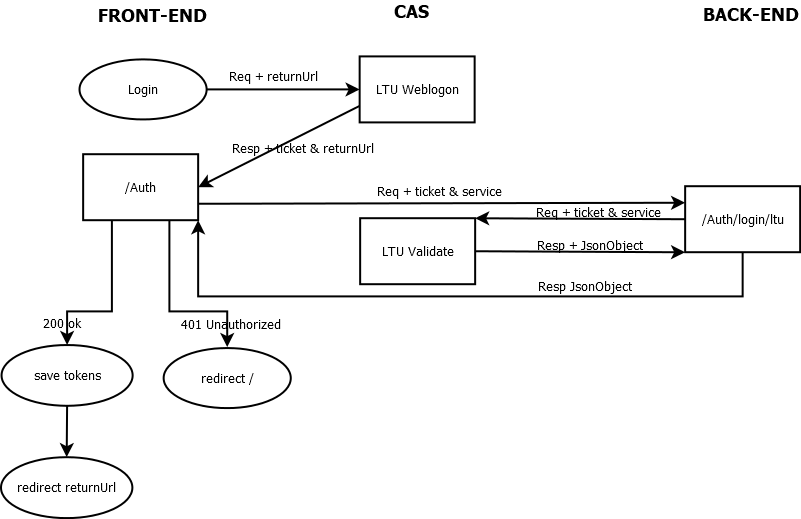
\includegraphics[width=\textwidth]{cas_login_flow.png}

\subsection{Auth interceptor}
The main purpose of this interceptor is to modify all requests by setting the authentication field in the header of the request for authenticated users. More than this it collects failed requests in the case of token expiration and tries to refresh the token to retry all failed requests automatically and stay logged in without the user being aware of affected.

\subsubsection{Technical}
even more technical?